%!TEX encoding = IsoLatin

%
% Chapitre "Fonctionnalites"
%

\chapter{Fonctionnalit�s}

\section{Image}

\section{Dessin vectoriel}

\section{Transformation}



\section{G�om�trie}



\subsection{Particules}

Pour respecter ce crit�re fonctionnel, l'application doit rendre un nuage de points en une seule commande d'affichage.

Dans l'application Paint3D+,  il y a un bouton nomm� ''Cloud Points'' qui permet de transformer un objet 3D s�lectionn� en  un nuage de points o� chaque point est un sommet d'unedes faces qui compose l'objet en 3D.

Donc, pour pouvoir utiliser cette option, il faut cr�er un objet 3D avec le bouton ''Cube'' ou ''Sphere'' en mode 3D, s�lectionner un des objets 3D cr�� avec le bouton ''Select next 3D Shape'' et appuyer sur le bouton ''Cloud Points'' pour rendre l'objet 3D s�lectionn� en tant que nuage de points.

Les 2 figures suivantes montrent une sph�re rendue sans nuage de points et une sph�re rendue avec un nuage de points.

\begin{figure}[h] 
\begin{center}
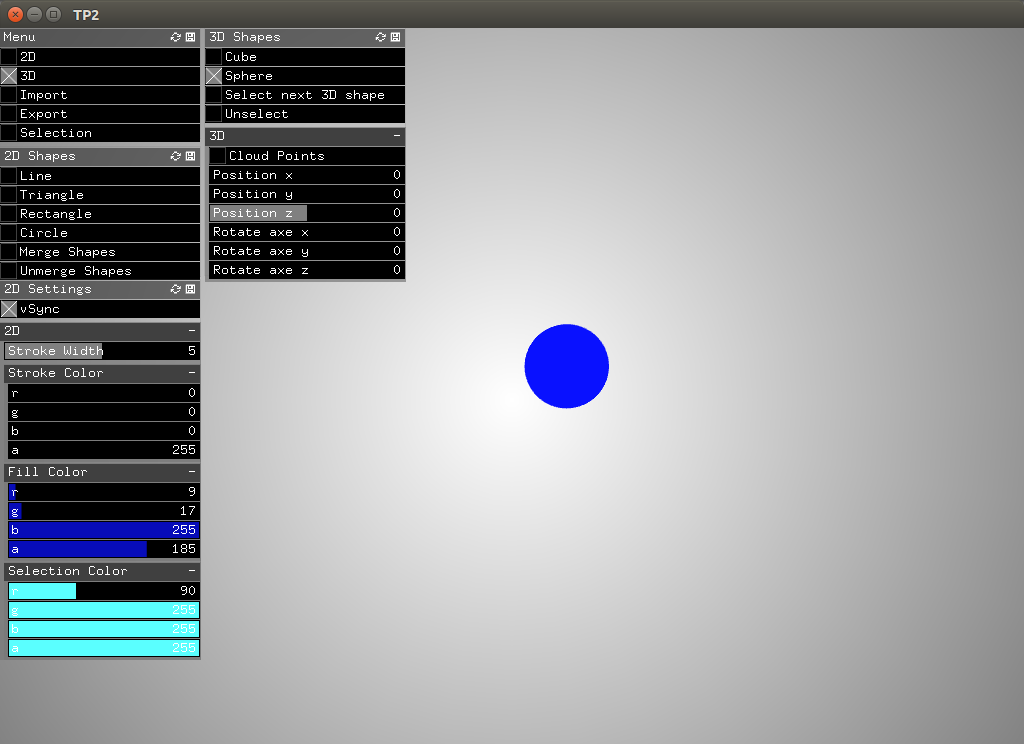
\includegraphics[width=13cm, height=13cm]{fig/cloudpoints1.png}
\end{center}
\caption{Une sph�re rendue sans nuage de points.}
\end{figure}
 
 
\begin{figure}[h] 
\begin{center}
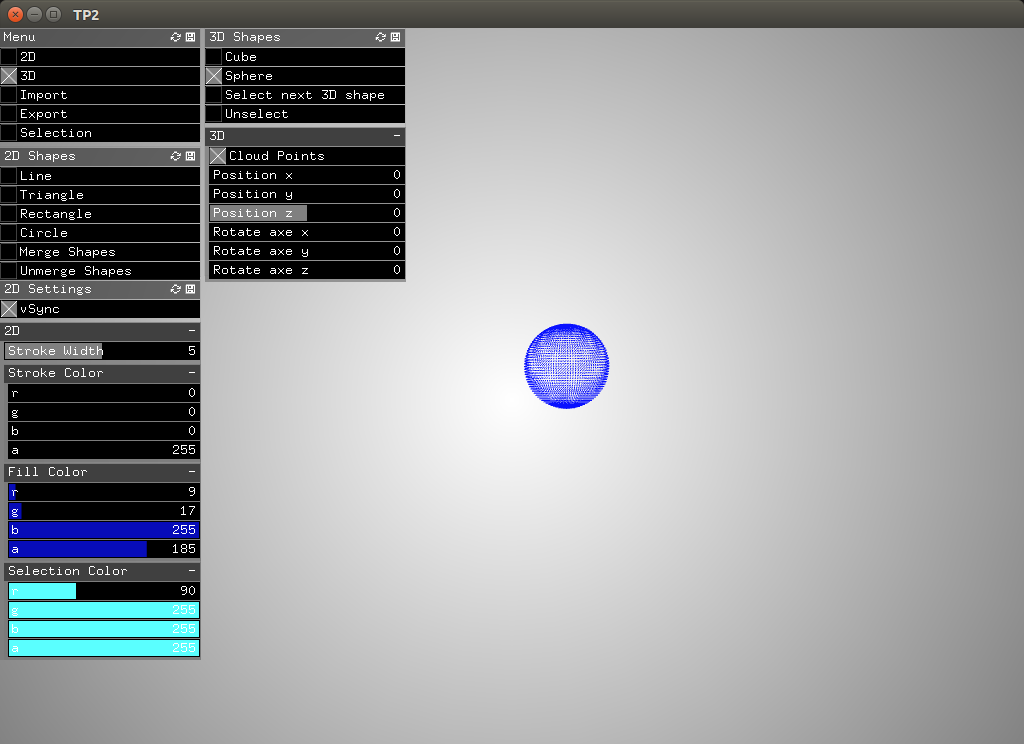
\includegraphics[width=13cm, height=13cm]{fig/cloudpoints2.png}
\end{center}
\caption{Une sph�re rendue avec un nuage de points.}
\end{figure}

\newpage

\subsection{Primitives 3D}

L'application doit permettre de cr�er au moins 2 types de primitives g�om�triques 3D � partir d'un algorithme sans aucune donn�es externes � l'application.

L'application Paint3D+ permet de cr�er 2 primitives 3D localement sans donn�es externes, soit le cube et la sph�re. Ces 2 primitives 3D sont cr��es par composition � partir de 2 classes d'OpenFrameworks, soit OfSpherePrimitive et OfxBoxPrimitive. 

Pour cr�er ces 2 primitives 3D, il faut d'abord s�lectionner le mode 3D dans le menu. Ensuite, il faut cocher soit Cube ou Sphere, selon la primitive 3D � cr�er et cliquer gauche sur la souris � l'endroit o� l'on veut que la primitive 3D apparaisse. Ensuite, pour modifier une primitive 3D cr��e, il faut la s�lectionner avec l'option ''Select next 3D shape'' et modifier les param�tres modifiables, soit la position en x,y,z l'orientation en x,y,z ou la couleur de s�lection ou de remplissage. 

Il est � noter que la rotation est faite � partir de quaternions dans le code.


\section{Illumination}

gggg
gggg
gggg
gg